% =====================================================================
% 4 RESULTS (describe only). Every number: analysis/RESULTS.md, cells.csv, cell_rates.csv, tests_refusal.csv,
% tests_capability.csv, correlations.csv, dev_matched_kl.csv, rank_flips.csv (assemble_p30.py, re-run 2026-11-06
% 22:47Z); supplementary statistics as computed by scripts/supp_stats.py.
% Seed-noise threshold quoted from paper 33: 33_2611_does_refusal_removal_get_harder/results/analysis/
% seednoise_summary.md (2 x SD_diff = 25.9 pp [18.1, 45.4]).
% Revised 2026-11-06: new 1.x cells lead; H1 = 1.x general vs 2.0 DiM; other configurations additional;
% H2 wording and figure caption corrected (no model showed the predicted crossover); H3 adds keyword-256;
% efficiency claim restricted to within-model evidence; selection-cap section labelled exploratory and suggestive.
% Revised 2026-11-06 (pm): 7B 1.x cells judged (H1 7B primary, H2 six models); KL <= 0.1 re-export answers the
% selection-cap question (families h1_kl_matched, kl_cap_1x); external tools (families vs_base_added,
% external_vs_heretic, external_sensitivity, kw_vs_judge_added). supp_stats.py was restricted to the 29
% original-design cells (as correlations.csv is) and re-run at 15:03 on the current analysis outputs; the supp_stats
% numbers below (within-model Spearman, keyword-256 counts, capped shares, H1 over-refusal by judge) match
% analysis/supp_stats.csv (checked 2026-11-06, integration pass).
% =====================================================================
\section{Results}
\label{sec:results}

% src (RESULTS.md "Coverage": 42 of 42 judged; "Anomalies and checks"; cells.csv wg_rate - wg_excl_adv_rate:
%      max 1.95 pp (qwen2.5-32b__dim), median 1.08 pp over the 29 main-design cells, 0.82 pp over all 42;
%      tests_refusal.csv harmful_all vs harmful_excl_advbench sig_holm: no change in vs_base, h1_1x_vs_2.0,
%      h1_kl_matched, kl_cap_1x, vs_base_added, external_sensitivity; external_vs_heretic: obliteratus-advanced vs
%      heretic1x-general (wg -4.6 [-7.7,-1.6] p=0.017 -> -3.1 [-6.2,-0.1] p=0.154) and three Qwen3Guard decisions)
The study asked which tool, version and method removes refusal best at the least capability cost when refusal is
judged on held-out prompts. Results are reported for the 29 cells of the main design (Table~\ref{tab:cells}) and
for the 13 added cells: the Qwen2.5-32B 1.x general search re-exported at the 2.0 selection rule
(\S\ref{sec:res-kl}, Table~\ref{tab:h1}) and the external tools with the Qwen3.5-4B context cells
(\S\ref{sec:res-external}, Table~\ref{tab:external}). All 42 cells passed the data checks
(Appendix~\ref{app:checks}). Excluding the 44 AdvBench-overlap prompts changed residual refusal by at most 1.95~pp
(median 1.08~pp in the main design) and left every edited-versus-original, 1.x-versus-2.0 and KL-matched decision
unchanged; among the external-tool contrasts it changed one WildGuard decision (\S\ref{sec:res-external}).

\begin{table*}[tbp]
\centering\footnotesize
\caption{Held-out results per cell of the main design and of the KL $\le$ 0.1 re-export ($^{\S}$, added after the
main design; also Table~\ref{tab:h1}b); the external-tool cells and the Qwen3.5-4B context are in
Table~\ref{tab:external}. Source: ``new'' = evaluated for this study; \cite{young2026harder} =
first reported in the companion study (responses and judge labels reused). WildGuard refusal: share of the 972
harmful prompts whose response WildGuard labels a refusal (Wilson 95\% CI). Change: paired difference from the same
model's original ($p_\mathrm{Holm}<0.001$ for 22 of the 23 changes of the main design; the exception is 1.x code on
Qwen2.5-7B, $p_\mathrm{Holm}=0.22$; the $^{\S}$ cell is tested in the separate family of added cells,
$p_\mathrm{Holm}<0.001$; for Qwen2.5-32B paired over the 971 prompts labelled in both models). Keyword: any of
Heretic~2.0's 33 default markers in the full response / in its first 256 tokens. HarmBench harmful: harmful
compliance by the HarmBench classifier. Over-refusal: WildGuard refusal on the 350 benign prompts. Capability
$\Delta$: change of the mean of the five benchmarks (pp). TF div.: teacher-forced divergence from the original on
the benign prompts (nats per token). SOM and J-space are plug-ins of the companion study's project fork, not part of
Heretic~2.0. The Qwen2.5-32B original was evaluated with an earlier harness revision (\S\ref{sec:procedure}).}
\label{tab:cells}
\setlength{\tabcolsep}{3.5pt}
\resizebox{\textwidth}{!}{\begin{tabular}{@{}lllrrrrrrrr@{}}
\toprule
Model & Condition & Source & \multicolumn{2}{c}{WildGuard refusal, harmful (\%)} & Change vs.\ & Keyword (\%) & HarmBench & Over-refusal & Capability & TF div. \\
 & & & rate & 95\% CI & original (pp) & full / 256 tok. & harmful (\%) & benign (\%) & $\Delta$ (pp) & (nats/tok.) \\
\midrule
Qwen2.5-7B & Original & \cite{young2026harder} & 72.1 & [69.2, 74.8] & -- & 75.8 / 74.5 & 23.3 & 4.3 & -- & -- \\
 & 1.x general & new & 39.6 & [36.6, 42.7] & $-$32.5 & 45.8 / 43.4 & 45.6 & 1.1 & $-$0.36 & 0.009 \\
 & 1.x code & new & 71.2 & [68.3, 74.0] & $-$0.9$^{\mathrm{ns}}$ & 71.9 / 71.4 & 25.5 & 5.1 & +0.80 & 0.075 \\
 & 2.0 DiM & \cite{young2026harder} & 20.6 & [18.2, 23.2] & $-$51.5 & 40.1 / 37.8 & 64.0 & 0.3 & +0.23 & 0.019 \\
 & 2.0 MPOA & \cite{young2026harder} & 13.8 & [11.8, 16.1] & $-$58.3 & 23.7 / 20.5 & 71.5 & 0.3 & $-$0.23 & 0.018 \\
 & SOM (fork plug-in) & \cite{young2026harder} & 12.2 & [10.3, 14.5] & $-$59.9 & 22.4 / 17.9 & 73.1 & 0.0 & $-$0.33 & 0.026 \\
 & J-space (fork plug-in) & \cite{young2026harder} & 52.6 & [49.4, 55.7] & $-$19.5 & 53.6 / 51.7 & 36.3 & 1.1 & +0.86 & 0.009 \\
 & 2.0 ARA & \cite{young2026harder} & 4.7 & [3.6, 6.3] & $-$67.4 & 16.6 / 11.0 & 79.0 & 0.0 & +0.48 & 0.048 \\
\addlinespace[2pt]
Qwen2.5-Coder-7B & Original & new & 83.2 & [80.8, 85.4] & -- & 83.6 / 83.5 & 15.4 & 22.6 & -- & -- \\
 & 1.x general & new & 10.3 & [8.5, 12.4] & $-$72.9 & 18.5 / 15.6 & 77.1 & 2.3 & $-$0.35 & 0.017 \\
 & 1.x code & new & 62.2 & [59.2, 65.2] & $-$21.0 & 62.3 / 61.8 & 33.4 & 7.1 & +0.24 & 0.008 \\
\addlinespace[2pt]
Qwen2.5-14B & Original & new & 77.6 & [74.8, 80.1] & -- & 78.0 / 77.2 & 18.8 & 4.0 & -- & -- \\
 & 1.x general & new & 58.2 & [55.1, 61.3] & $-$19.3 & 63.6 / 61.8 & 30.6 & 0.3 & $-$0.13 & 0.018 \\
 & 1.x code & new & 75.0 & [72.2, 77.6] & $-$2.6 & 73.6 / 73.1 & 20.1 & 3.7 & $-$0.15 & 0.006 \\
\addlinespace[2pt]
Qwen2.5-Coder-14B & Original & new & 85.5 & [83.1, 87.6] & -- & 85.2 / 85.0 & 13.9 & 17.4 & -- & -- \\
 & 1.x general & new & 12.3 & [10.4, 14.6] & $-$73.1 & 21.7 / 18.4 & 76.1 & 0.9 & +0.24 & 0.020 \\
 & 1.x code & new & 77.2 & [74.4, 79.7] & $-$8.3 & 75.8 / 75.5 & 20.5 & 8.0 & +0.47 & 0.007 \\
\addlinespace[2pt]
Qwen2.5-32B & Original & \cite{young2026harder} & 76.8 & [74.1, 79.4] & -- & 76.4 / 75.9 & 19.8 & 5.1 & -- & -- \\
 & 1.x general & new & 73.4 & [70.5, 76.0] & $-$3.4 & 72.9 / 72.1 & 22.1 & 2.3 & +0.19 & 0.007 \\
 & 1.x general, KL $\le$ 0.1$^{\ddagger}$ & new & 11.6 & [9.8, 13.8] & $-$65.2 & 28.2 / 24.2 & 74.6 & 0.0 & +0.02 & 0.032 \\
 & 1.x code & new & 65.3 & [62.3, 68.3] & $-$11.4 & 62.8 / 61.3 & 27.6 & 0.6 & $-$0.25 & 0.017 \\
 & 2.0 DiM & \cite{young2026harder} & 47.4 & [44.3, 50.6] & $-$29.4 & 55.3 / 52.5 & 40.3 & 0.6 & $-$0.05 & 0.017 \\
 & 2.0 MPOA & \cite{young2026harder} & 3.9 & [2.9, 5.3] & $-$72.9 & 17.1 / 12.3 & 85.3 & 0.0 & $-$0.03 & 0.042 \\
 & SOM (fork plug-in) & \cite{young2026harder} & 42.7 & [39.6, 45.8] & $-$34.1 & 46.9 / 43.7 & 44.5 & 0.6 & +0.31 & 0.020 \\
 & 2.0 ARA & \cite{young2026harder} & 6.1 & [4.7, 7.8] & $-$70.8 & 19.1 / 14.2 & 82.3 & 0.0 & $-$0.83 & 0.077 \\
 & huihui-ai & \cite{young2026harder} & 1.3 & [0.8, 2.3] & $-$75.5 & 8.2 / 6.3 & 90.1 & 0.0 & $-$0.94 & 0.151 \\
 & zetasepic v2 & \cite{young2026harder} & 1.1 & [0.6, 2.0] & $-$75.7 & 12.9 / 8.8 & 91.0 & 0.0 & $-$0.45 & 0.085 \\
\addlinespace[2pt]
Qwen2.5-Coder-32B & Original & new & 75.3 & [72.5, 77.9] & -- & 77.0 / 76.3 & 19.9 & 4.3 & -- & -- \\
 & 1.x general & new & 64.3 & [61.2, 67.3] & $-$11.0 & 70.5 / 69.3 & 28.7 & 2.0 & +0.50 & 0.004 \\
 & 1.x code & new & 61.1 & [58.0, 64.1] & $-$14.2 & 69.3 / 67.7 & 30.7 & 1.1 & +0.29 & 0.004 \\
\bottomrule
\multicolumn{11}{@{}l}{\footnotesize $^{\ddagger}$ Added after the pre-stated design: the original 1.x general study re-exported at the 2.0 selection rule (dev KL $\le$ 0.1; trial \#96); its test is in a separate Holm family.} \\
\multicolumn{11}{@{}l}{\footnotesize $^{\mathrm{ns}}$ $p_\mathrm{Holm} \ge 0.05$; all other changes $p_\mathrm{Holm} < 0.001$. External tools and Qwen3.5-4B: Table~\ref{tab:external}.} \\
\end{tabular}
}
\end{table*}

\subsection{Heretic 1.x on Six Qwen2.5 Models}

% src (RESULTS.md "Modified vs original (family vs_base ...)"; tests_refusal.csv family vs_base: wg 22/23 sig,
%      kw 23/23, q3g 23/23, benign wg 21/23 (ns: 7b 1.x code p=0.906, 14b 1.x code p=1.00); cells.csv
%      dev_refusals, tf_divergence, capability_mean_delta_pp/_lo/_hi, overrefusal_wg_rate)
Every edited model of the main design refused significantly less than its original under keyword matching and
Qwen3Guard (23 of 23 comparisons each), and all but one did so under WildGuard (22 of 23; Table~\ref{tab:cells},
Figure~\ref{fig:refusal}a). The exception was the 1.x code variant on Qwen2.5-7B, which left 71.2\% of the harmful
prompts refused against 72.1\% for its original ($-$0.9~pp [$-$2.3, +0.4], $p_\mathrm{Holm}=0.22$); under keyword
matching and Qwen3Guard its reductions were 3.9 and 2.2~pp. The six originals refused 72.1\% (Qwen2.5-7B) to
85.5\% (Qwen2.5-Coder-14B) of the harmful prompts. The same 1.x procedure removed very different amounts of refusal
on different models: 32.5~pp (general variant) and 0.9~pp (code variant) on Qwen2.5-7B, 72.9~pp and 21.0~pp on
Qwen2.5-Coder-7B, 19.3~pp and 2.6~pp on Qwen2.5-14B, 73.1~pp and 8.3~pp on Qwen2.5-Coder-14B, 3.4~pp and 11.4~pp on
Qwen2.5-32B, and 11.0~pp and 14.2~pp on Qwen2.5-Coder-32B. The selected 1.x general trials had kept 67, 21, 91, 36,
89 and 94 of 100 dev refusals on these six models. Eleven of the twelve 1.x models diverged little from their
originals (TF divergence 0.004 to 0.020 nats per token); the exception was 1.x code on Qwen2.5-7B (0.075). Their
mean capability changes ranged from $-$0.36 to +0.80~pp, with every interval including zero, and over-refusal on the
benign prompts fell significantly (Holm) in ten of them, for example from 22.6\% to 2.3\% (general) and 7.1\% (code)
on Qwen2.5-Coder-7B; the exceptions were 1.x code on Qwen2.5-7B (5.1\% vs.\ 4.3\%, $p_\mathrm{Holm}=0.91$) and on
Qwen2.5-14B (3.7\% vs.\ 4.0\%, $p_\mathrm{Holm}=1.00$).

For comparison, the companion-study cells on Qwen2.5-32B, the only model on which all tool families were evaluated,
left 1.1\% (zetasepic v2), 1.3\% (huihui-ai), 3.9\% (2.0 MPOA), 6.1\% (2.0 ARA), 42.7\% (SOM, fork plug-in) and
47.4\% (2.0 DiM) of the harmful prompts refused, against 76.8\% for the original. On Qwen2.5-7B the 2.0 methods and
fork plug-ins left 4.7\% (ARA), 12.2\% (SOM, fork plug-in), 13.8\% (MPOA), 20.6\% (DiM) and 52.6\% (J-space,
fork plug-in) against 72.1\%.

\begin{figure*}[tbp]
\centering
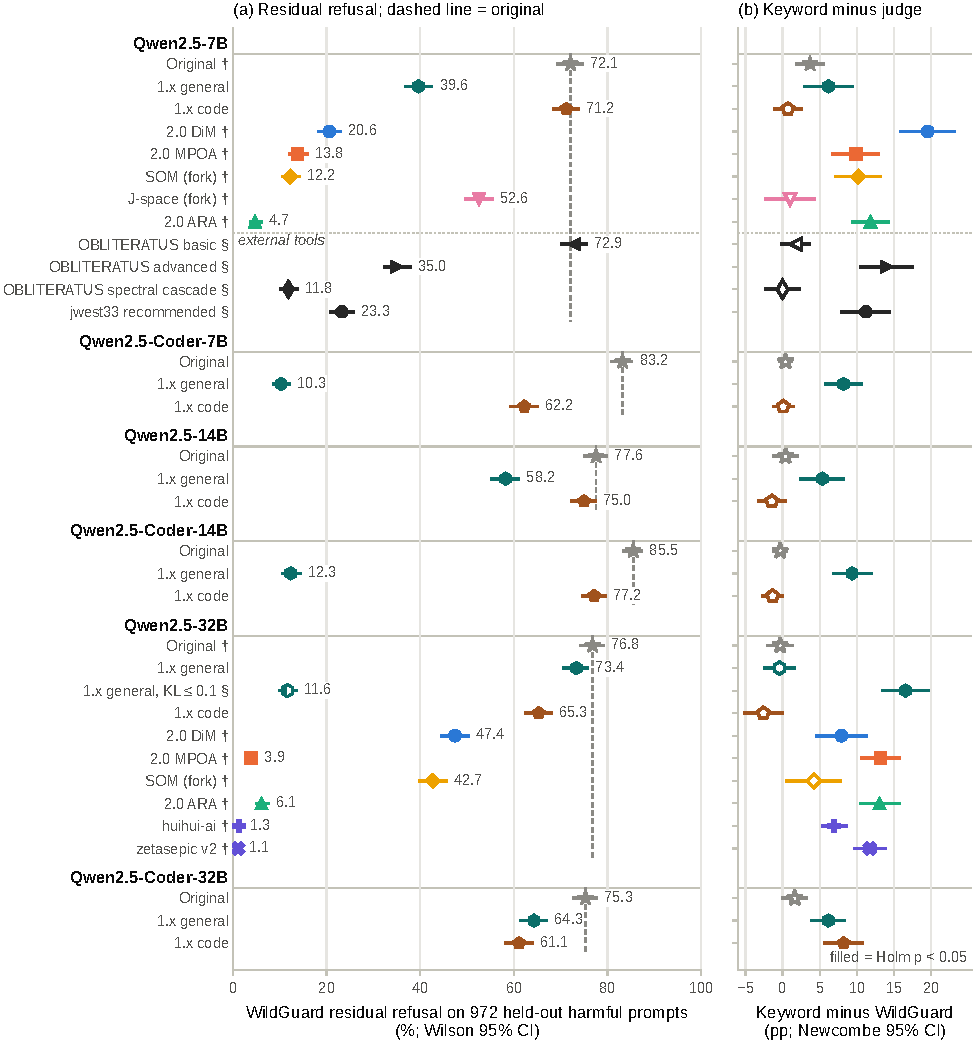
\includegraphics[width=\textwidth]{figures/fig1_residual_refusal.pdf}
\caption{\textbf{Residual refusal by model and condition (held-out, judged; Qwen2.5 models).} (a) Share of the 972
harmful held-out prompts whose response WildGuard labels a refusal, with Wilson 95\% intervals; the dashed line marks
the model's original. (b) Keyword refusal rate minus WildGuard refusal rate on the same responses, with Newcombe 95\%
intervals; filled markers are significant after Holm correction, over the 29 cells of the main design and separately
over the 13 added cells. $\S$ = cell added after the main design (the KL $\le$ 0.1 re-export on Qwen2.5-32B and the
external tools on Qwen2.5-7B, run once at their own settings); the Qwen3.5-4B cells are in
Figure~\ref{fig:tradeoff}c,d and Table~\ref{tab:external}. Heretic~1.x
(teal hexagons, sienna pentagons) was selected at dev KL $\le$ 0.01 (half-filled hexagon: the re-export at dev KL
$\le$ 0.1), Heretic~2.0 and the fork plug-ins at dev KL $\le$ 0.1; ``(fork)'' marks plug-ins of the companion study's project fork, not part of Heretic~2.0; the community
releases are public Qwen2.5-32B abliterations. $\dagger$ = cell first reported in the companion study
\cite{young2026harder}.}
\label{fig:refusal}
\end{figure*}

\subsection{Like-for-Like Version Contrast (H1)}

% src (RESULTS.md "H1 -- Heretic 1.x vs Heretic 2.0 on the same base"; tests_refusal.csv family h1_1x_vs_2.0
%      (n_in_family 18) judges wg/kw/q3g, groups harmful_all/harmful_excl_advbench/benign_all; cells.csv dev_*,
%      tf_divergence, capability_mean_delta_*; supp_stats logic: h1 over-refusal 32B primary wg 2.3 vs 0.6 p=0.773,
%      kw 13.1 vs 12.0 p=1.000, q3g 5.1 vs 2.6 p=0.043; 32B family: wg 0/8, kw 2/8, q3g 3/8)
In the like-for-like contrast on Qwen2.5-32B, 1.x general left 73.4\% of the harmful prompts refused and 2.0 DiM
47.4\%, a paired difference of +25.9~pp [23.0, 28.7]; 259 prompts were refused by the 1.x model only and 7 by the
DiM model only ($p_\mathrm{Holm}<0.001$; Table~\ref{tab:h1}). The difference remained significant under keyword
matching, under Qwen3Guard and without the AdvBench-overlap prompts. Both released trials had kept 89 of 100 dev
refusals, at a dev KL of 0.006 (1.x) and 0.018 (DiM) and a TF divergence of 0.007 and 0.017 nats per token. Neither
model changed capability measurably (mean change +0.19~pp [$-$1.06, +1.45] for 1.x general and $-$0.05~pp
[$-$1.35, +1.25] for DiM). Over-refusal did not differ under WildGuard (2.3\% vs.\ 0.6\%, $p_\mathrm{Holm}=0.77$)
or keyword matching (13.1\% vs.\ 12.0\%, $p_\mathrm{Holm}=1.00$) but was higher for 1.x under Qwen3Guard (5.1\% vs.\
2.6\%, $p_\mathrm{Holm}=0.043$). The difference equals the threshold of two standard deviations of the difference
between two independently optimised cells that the companion study estimated from seed replicates of its
Qwen2.5-7B and Qwen3.5-4B cells (25.9~pp [18.1, 45.4]) \cite{young2026harder}.

% src (tests_refusal.csv h1_1x_vs_2.0, model qwen2.5-7b: general vs dim wg +19.0 [16.1,21.9] 215/30; kw +5.7
%      [2.5,8.8] p=0.0005; q3g +21.2 [18.3,24.0]; excl adv +17.7 [14.7,20.6]; benign wg 1.1 vs 0.3, kw 7.7 vs 8.3,
%      q3g 2.6 vs 1.7, all p_holm=1; cells.csv: 7B 1.x general dev 67 @ 0.0053, tf 0.0089, cap -0.36 [-1.35,0.63];
%      7B dim dev 55 @ 0.0782, tf 0.0194, cap +0.23 [-0.85,1.32])
On Qwen2.5-7B, 1.x general left 39.6\% [36.6, 42.7] of the harmful prompts refused and 2.0 DiM 20.6\% [18.2, 23.2],
a paired difference of +19.0~pp [16.1, 21.9]; 215 prompts were refused by the 1.x model only and 30 by the DiM model
only ($p_\mathrm{Holm}<0.001$). The difference remained significant under keyword matching (+5.7~pp [2.5, 8.8],
$p_\mathrm{Holm}<0.001$), under Qwen3Guard (+21.2~pp [18.3, 24.0]) and without the AdvBench-overlap prompts
(+17.7~pp [14.7, 20.6]). The released 1.x trial had kept 67 of 100 dev refusals at a dev KL of 0.005, the DiM trial
55 at 0.078; their TF divergences were 0.009 and 0.019 nats per token. Neither model changed capability measurably
($-$0.36~pp [$-$1.35, +0.63] and +0.23~pp [$-$0.85, +1.32]), and over-refusal did not differ under any judge
(WildGuard 1.1\% vs.\ 0.3\%, keyword matching 7.7\% vs.\ 8.3\%, Qwen3Guard 2.6\% vs.\ 1.7\%; $p_\mathrm{Holm}=1.00$
each). H1 was therefore supported for the released checkpoints on both base models: on Qwen2.5-32B by a difference
equal to the companion study's seed-noise threshold and on Qwen2.5-7B by a difference below it.
Section~\ref{sec:res-kl} repeats the Qwen2.5-32B contrast with both arms selected by the same rule.

% src (tests_refusal.csv h1_1x_vs_2.0: 32B 8/8 and 7B 10/10 significant under wg, kw, q3g and harmful_excl_advbench
%      with identical signs; benign: 7B wg 5/10 (all 1.x code), kw 2/10 (1.x code vs mpoa, som), q3g 5/10 (all 1.x
%      code); tests_capability.csv original_design: 0 of 115 Holm-significant, min p 0.0166 (7b 1.x code gsm8k
%      +3.2 [0.7,5.8]), next 0.0215 (32b ara humaneval -4.9 [-9.3,-0.9]))
The additional configurations on Qwen2.5-32B all left less residual refusal than both released 1.x variants
(selected at dev KL $\le$ 0.01; \S\ref{sec:res-kl}): 1.x general
exceeded SOM (fork plug-in) by 30.7~pp, ARA by 67.3~pp and MPOA by 69.4~pp [66.4, 72.2], and 1.x code exceeded the
four configurations by 17.9 to 61.4~pp. The discordant prompts ran almost entirely in one direction; for example, 675
prompts were refused by 1.x general and not by MPOA, and none the other way. On Qwen2.5-7B, 1.x general left more
residual refusal than MPOA (+25.8~pp [22.8, 28.8]), SOM (+27.4~pp [24.4, 30.3]) and ARA (+34.9~pp [31.8, 37.9]) and
less than J-space (fork plug-in; $-$13.0~pp [$-$15.6, $-$10.3]; 32 versus 158 discordant prompts); 1.x code, which
had removed no significant refusal, exceeded all five configurations, by 18.6~pp (J-space) to 66.5~pp (ARA). All 18
contrasts were significant ($p_\mathrm{Holm}<0.001$) with the same sign under WildGuard, keyword matching and
Qwen3Guard and without the AdvBench-overlap prompts. Over-refusal differed in none of the Qwen2.5-32B contrasts under
WildGuard, in two under keyword matching and in three under Qwen3Guard (including the primary contrast); on
Qwen2.5-7B it differed only in contrasts of 1.x code (five under WildGuard and Qwen3Guard, two under keyword
matching), whose 5.1\% WildGuard over-refusal exceeded the 0.0--1.1\% of the 2.0 and fork models. No per-benchmark
capability change of any edited model of the main design was significant after Holm correction (115 tests; the
smallest unadjusted $p$ was 0.017, for a GSM8K gain of +3.2~pp [0.7, 5.8] after 1.x code on Qwen2.5-7B, followed by
0.021 for a HumanEval change of $-$4.9~pp [$-$9.3, $-$0.9] after 2.0 ARA on Qwen2.5-32B;
Appendix~\ref{app:capability}).

% KL-matched rows are panel (b) of tables/tab_h1.tex (checked 2026-11-06); no separate tab:h1-kl.
\begin{table*}[tbp]
\centering\small
\caption{H1: Heretic~1.x versus Heretic~2.0 and fork plug-ins on the same base model (WildGuard residual refusal on
the 972 harmful prompts). Primary = like-for-like contrast (1.x general versus 2.0 DiM, the same edit;
Table~\ref{tab:h1setup}); additional = configurations that also change the edit. ``(fork)'' = plug-in of the
companion study's project fork, not part of Heretic~2.0. Differences are paired (Newcombe 95\% CI); 1.x-only /
comp.-only are prompts refused by one model only; $p_\mathrm{Holm}$ from exact McNemar tests; the last column
repeats the test with keyword matching. (a) Released trials, Holm over the 18 1.x-versus-2.0 contrasts
(conservative for the primary contrasts). (b) Added after the main results: trial~\#96 of the archived Qwen2.5-32B
1.x general search, re-exported at the 2.0 selection rule (\S\ref{sec:reexport}), against the same comparators
(KL-matched, Holm over these four contrasts) and against the released trial~\#84 of the same search (cap only, a
single unadjusted test).}
\label{tab:h1}
\setlength{\tabcolsep}{4pt}
\resizebox{\textwidth}{!}{\begin{tabular}{@{}llllrrrrrr@{}}
\toprule
Model & Contrast & 1.x variant & Comparator & 1.x (\%) & Comparator (\%) & 1.x $-$ comparator (pp) [95\% CI] & 1.x-only / comp.-only & $p_\mathrm{Holm}$ & keyword $p_\mathrm{Holm}$ \\
\midrule
\multicolumn{10}{@{}l}{\textit{(a) Pre-stated design: released trials (1.x selected at dev KL $\le$ 0.01, 2.0 and fork at dev KL $\le$ 0.1); Holm over the 18 contrasts}} \\
\addlinespace[1pt]
Qwen2.5-32B & primary & general & 2.0 DiM & 73.4 & 47.4 & +25.9 [+23.0, +28.7] & 259 / 7 & $<$0.001 & $<$0.001 \\
\addlinespace[1pt]
 & additional & general & 2.0 MPOA & 73.4 & 3.9 & +69.4 [+66.4, +72.2] & 675 / 0 & $<$0.001 & $<$0.001 \\
 & additional & general & 2.0 ARA & 73.4 & 6.1 & +67.3 [+64.2, +70.1] & 655 / 1 & $<$0.001 & $<$0.001 \\
 & additional & general & SOM (fork) & 73.4 & 42.7 & +30.7 [+27.7, +33.5] & 300 / 2 & $<$0.001 & $<$0.001 \\
 & additional & code & 2.0 DiM & 65.3 & 47.4 & +17.9 [+15.3, +20.4] & 183 / 9 & $<$0.001 & $<$0.001 \\
 & additional & code & 2.0 MPOA & 65.3 & 3.9 & +61.4 [+58.2, +64.4] & 599 / 2 & $<$0.001 & $<$0.001 \\
 & additional & code & 2.0 ARA & 65.3 & 6.1 & +59.3 [+55.9, +62.4] & 585 / 9 & $<$0.001 & $<$0.001 \\
 & additional & code & SOM (fork) & 65.3 & 42.7 & +22.6 [+19.8, +25.3] & 228 / 8 & $<$0.001 & $<$0.001 \\
\addlinespace[2pt]
Qwen2.5-7B & primary & general & 2.0 DiM & 39.6 & 20.6 & +19.0 [+16.1, +21.9] & 215 / 30 & $<$0.001 & $<$0.001 \\
\addlinespace[1pt]
 & additional & general & 2.0 MPOA & 39.6 & 13.8 & +25.8 [+22.8, +28.8] & 269 / 18 & $<$0.001 & $<$0.001 \\
 & additional & general & 2.0 ARA & 39.6 & 4.7 & +34.9 [+31.8, +37.9] & 344 / 5 & $<$0.001 & $<$0.001 \\
 & additional & general & SOM (fork) & 39.6 & 12.2 & +27.4 [+24.4, +30.3] & 278 / 12 & $<$0.001 & $<$0.001 \\
 & additional & general & J-space (fork) & 39.6 & 52.6 & $-$13.0 [$-$15.6, $-$10.3] & 32 / 158 & $<$0.001 & $<$0.001 \\
 & additional & code & 2.0 DiM & 71.2 & 20.6 & +50.6 [+47.3, +53.7] & 495 / 3 & $<$0.001 & $<$0.001 \\
 & additional & code & 2.0 MPOA & 71.2 & 13.8 & +57.4 [+54.1, +60.4] & 561 / 3 & $<$0.001 & $<$0.001 \\
 & additional & code & 2.0 ARA & 71.2 & 4.7 & +66.5 [+63.3, +69.3] & 647 / 1 & $<$0.001 & $<$0.001 \\
 & additional & code & SOM (fork) & 71.2 & 12.2 & +59.0 [+55.7, +61.9] & 574 / 1 & $<$0.001 & $<$0.001 \\
 & additional & code & J-space (fork) & 71.2 & 52.6 & +18.6 [+16.0, +21.2] & 189 / 8 & $<$0.001 & $<$0.001 \\
\midrule
\multicolumn{10}{@{}l}{\textit{(b) Added: the original 1.x general study re-exported at the 2.0 selection rule (dev KL $\le$ 0.1; trial \#96); separate Holm families}} \\
\addlinespace[1pt]
Qwen2.5-32B & KL-matched & general, \#96 & 2.0 DiM & 11.6 & 47.4 & $-$35.8 [$-$38.9, $-$32.7] & 5 / 353 & $<$0.001 & $<$0.001 \\
 & KL-matched & general, \#96 & 2.0 MPOA & 11.6 & 3.9 & +7.7 [+5.9, +9.7] & 83 / 8 & $<$0.001 & $<$0.001 \\
 & KL-matched & general, \#96 & 2.0 ARA & 11.6 & 6.1 & +5.6 [+3.6, +7.6] & 77 / 23 & $<$0.001 & $<$0.001 \\
 & KL-matched & general, \#96 & SOM (fork) & 11.6 & 42.7 & $-$31.1 [$-$34.0, $-$28.1] & 6 / 308 & $<$0.001 & $<$0.001 \\
\addlinespace[1pt]
 & cap only & general, \#96 & general, \#84 & 11.6 & 73.4 & $-$61.7 [$-$64.7, $-$58.5] & 2 / 602 & $<$0.001 & $<$0.001 \\
\bottomrule
\multicolumn{10}{@{}l}{\footnotesize Panel (b): KL-matched rows, Holm over 4 contrasts (family \texttt{h1\_kl\_matched}); cap-only row, a single test (family \texttt{kl\_cap\_1x}).} \\
\multicolumn{10}{@{}l}{\footnotesize \#84: the released 1.x general model of panel (a) (dev KL 0.006); \#96: fewest dev refusals at dev KL $\le$ 0.1 (KL 0.064); same study, journal and heretic-llm 1.4.0.} \\
\multicolumn{10}{@{}l}{\footnotesize KL-matched: both sides selected by the same rule (fewest dev refusals at dev KL $\le$ 0.1); realised dev KL still differs (Table~\ref{tab:devkl}). One optimisation run per condition.} \\
\end{tabular}
}
\end{table*}

\subsection{Like-for-Like Contrast at the Same Selection Rule}
\label{sec:res-kl}

% src (RESULTS.md "1.x general re-exported at KL <= 0.1 (trial #96) vs Heretic 2.0" and "1.x general at KL <= 0.1
%      vs the original 1.x export at KL <= 0.01"; tests_refusal.csv families h1_kl_matched (n_in_family 4) and
%      kl_cap_1x (1): wg/kw/q3g/excl-adv all same sign and p_holm < 0.001; kw: dim -27.2, som -18.7, mpoa +11.1,
%      ara +9.1; seed-noise threshold: paper 33 seednoise_summary.md)
The 1.x general model selected by the 2.0 rule from the archived Qwen2.5-32B search (trial~\#96;
\S\ref{sec:reexport}) left 11.6\% [9.8, 13.8] of the harmful prompts refused, against 73.4\% for the released
export of the same search (dev KL $\le$ 0.01) and 76.8\% for the original (Table~\ref{tab:h1}). The paired
difference between the two exports of the same search was $-$61.7~pp [$-$64.7, $-$58.5]: 602 prompts were refused
only by the KL $\le$ 0.01 export and 2 only by the KL $\le$ 0.1 export ($p<0.001$). Against the configurations on
the same base model, the KL $\le$ 0.1 export left 35.8~pp [32.7, 38.9] less residual refusal than 2.0 DiM (5 versus
353 discordant prompts) and 31.1~pp [28.1, 34.0] less than SOM (fork plug-in), and 7.7~pp [5.9, 9.7] more than MPOA
(83 versus 8) and 5.6~pp [3.6, 7.6] more than ARA (77 versus 23); all four $p_\mathrm{Holm}<0.001$. Each contrast
had the same sign and remained significant under keyword matching, under Qwen3Guard and without the AdvBench-overlap
prompts. With both arms of the like-for-like contrast selected by the same rule, the order therefore reversed: the
1.x general model left less residual refusal than 2.0 DiM, by a difference larger than the companion study's
seed-noise threshold (25.9~pp [18.1, 45.4]). This comparison rests on one search per arm (one seed each) on one base
model, and the two arms still differed in trial budget, search seed, optimisation system prompt and marker list
(Table~\ref{tab:h1setup}).

% src (cells.csv qwen2.5-32b__heretic1x-general-kl0.1: dev 50 @ 0.0642, reeval 51 @ 0.0637, tf 0.0323,
%      capability +0.02 [-1.27,1.31], overrefusal_wg 0.0, hb_harm 0.746, degenerate 1/972, kw 28.2; tf of
%      qwen2.5-32b__{heretic1x-general 0.0066, dim 0.0165, som 0.0202, mpoa 0.0416, ara 0.0773}; hb_harm 1.x 0.221,
%      dim 0.403; tests_capability.csv added: none Holm-significant; kl_cap_1x benign wg -2.3 [-4.4,-0.7] p=0.0078;
%      kw_vs_judge_added: +16.6 [13.4,19.7])
The KL $\le$ 0.1 export moved the model further than the released 1.x export, DiM and SOM but less than MPOA and
ARA: its TF divergence was 0.032 nats per token, against 0.007 for the KL $\le$ 0.01 export, 0.017 for DiM, 0.020 for SOM,
0.042 for MPOA and 0.077 for ARA. Its mean capability change was +0.02~pp [$-$1.27, +1.31], and no benchmark change
was significant. WildGuard over-refusal on the benign prompts was 0.0\%, against 2.3\% for the KL $\le$ 0.01 export
($-$2.3~pp [$-$4.4, $-$0.7], $p=0.008$); harmful compliance by the HarmBench classifier was 74.6\%, against 22.1\%
for the KL $\le$ 0.01 export and 40.3\% for DiM; and 1 of its 972 harmful responses was degenerate. Keyword matching
counted 28.2\% of its harmful responses as refusals, 16.6~pp [13.4, 19.7] more than WildGuard. No KL-matched cell
exists for the 1.x code variant or for Qwen2.5-7B (\S\ref{sec:reexport}).

\subsection{Source of the Refusal Direction (H2)}

% src (RESULTS.md "H2 -- 1.x general vs 1.x code, by item group"; tests_refusal.csv h2_general_vs_code (n_in_family
%      6); cells.csv wg_code_rate / wg_noncode_rate of the six originals (code 13.5-34.0, non-code 87.3-98.8);
%      tf_divergence of the 12 1.x cells)
The originals refused only 13.5\% (Qwen2.5-7B) to 34.0\% (Qwen2.5-Coder-14B) of the code-as-weapon prompts,
against 87.3\% to 98.8\% of the other harmful prompts (Figure~\ref{fig:general-code}). H2 predicted a crossover: the
code variant lower than the general variant on code-as-weapon prompts and higher on non-code prompts. No model showed
this crossover (Table~\ref{tab:h2}). On Qwen2.5-7B, Qwen2.5-Coder-7B, Qwen2.5-14B and Qwen2.5-Coder-14B the code
variant left more residual refusal on both subsets (code-as-weapon 12.0\% vs.\ 2.0\%, 8.0\% vs.\ 0.5\%, 14.5\% vs.\
5.5\% and 16.0\% vs.\ 0.0\%; non-code 86.5\% vs.\ 49.4\%, 76.3\% vs.\ 12.8\%, 90.7\% vs.\ 71.9\% and 93.0\% vs.\
15.5\%). Without the 41 prompts drawn from the code variant's source corpora, the code-as-weapon differences on
Qwen2.5-7B ($-$6.3~pp [$-$11.3, $-$2.5], $p_\mathrm{Holm}=0.010$) and on both 14B models remained significant and
that on Qwen2.5-Coder-7B did not ($-$3.8~pp [$-$8.0, $-$0.7], $p_\mathrm{Holm}=0.094$). On Qwen2.5-32B the code
variant left less on both subsets (code-as-weapon 6.5\% vs.\ 12.0\%; non-code 80.6\% vs.\ 89.2\%), and without the
41 prompts the code-as-weapon difference was +3.1~pp [$-$0.5, +7.4] ($p_\mathrm{Holm}=0.250$). On
Qwen2.5-Coder-32B the code variant left less on non-code prompts (74.6\% vs.\ 78.6\%) and the same on code-as-weapon
prompts (9.0\% each). In all six models, the variant that left less residual refusal on one subset left less or equal
residual refusal on the other. The code variant's released models diverged less from their originals than the
general variant's on Qwen2.5-Coder-7B and both 14B models (TF divergence 0.008, 0.006 and 0.007 vs.\ 0.017, 0.018
and 0.020 nats per token), more on Qwen2.5-7B (0.075 vs.\ 0.009) and Qwen2.5-32B (0.017 vs.\ 0.007) and equally on
Qwen2.5-Coder-32B (0.004 each). H2 was not supported.

\begin{figure}[tbp]
\centering
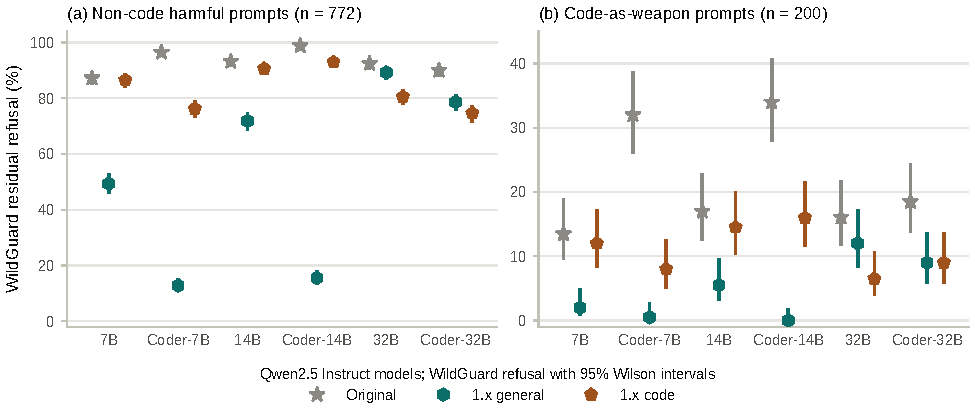
\includegraphics[width=\textwidth]{figures/fig3_general_vs_code.pdf}
\caption{\textbf{Heretic~1.x general versus code variant (H2).} WildGuard residual refusal with Wilson 95\%
intervals for the original (grey star), the 1.x general variant (direction from \texttt{harmful\_behaviors} versus
\texttt{harmless\_alpaca}) and the 1.x code variant (direction from malicious- versus benign-code prompts) on
(a) the 772 non-code harmful prompts and (b) the 200 code-as-weapon prompts; the panels use different vertical
scales. H2 predicted the code variant to be lower in (b) and higher in (a). No model showed this crossover: the code
variant was higher in both panels on the two 7B and the two 14B models, lower in both on Qwen2.5-32B (in (b) not
significantly once the 41 prompts from its source corpora are excluded) and lower in (a) and equal in (b) on
Qwen2.5-Coder-32B.}
\label{fig:general-code}
\end{figure}

\begin{table}[tbp]
\centering\small
\caption{H2: Heretic~1.x general versus code variant by prompt subset (WildGuard residual refusal; paired
Newcombe 95\% CI; exact McNemar, Holm over the six models within each subset). A negative difference means that
the general variant left less residual refusal.}
\label{tab:h2}
\setlength{\tabcolsep}{3pt}
\resizebox{\textwidth}{!}{\begin{tabular}{@{}llrrrr@{}}
\toprule
Model & Prompt subset ($n$) & General (\%) & Code (\%) & General $-$ code (pp) [95\% CI]; $<0$: general lower & $p_\mathrm{Holm}$ \\
\midrule
Qwen2.5-7B & Non-code harmful (772) & 49.4 & 86.5 & $-$37.2 [$-$40.6, $-$33.7] & $<$0.001 \\
 & Code-as-weapon (200) & 2.0 & 12.0 & $-$10.0 [$-$15.0, $-$6.0] & $<$0.001 \\
 & Code-as-weapon, excl.\ RMCBench/MalwareBench (159) & 1.9 & 8.2 & $-$6.3 [$-$11.3, $-$2.5] & 0.010 \\
\addlinespace[2pt]
Qwen2.5-Coder-7B & Non-code harmful (772) & 12.8 & 76.3 & $-$63.5 [$-$66.8, $-$59.8] & $<$0.001 \\
 & Code-as-weapon (200) & 0.5 & 8.0 & $-$7.5 [$-$12.1, $-$3.9] & $<$0.001 \\
 & Code-as-weapon, excl.\ RMCBench/MalwareBench (159) & 0.0 & 3.8 & $-$3.8 [$-$8.0, $-$0.7] & 0.094 \\
\addlinespace[2pt]
Qwen2.5-14B & Non-code harmful (772) & 71.9 & 90.7 & $-$18.8 [$-$21.7, $-$16.0] & $<$0.001 \\
 & Code-as-weapon (200) & 5.5 & 14.5 & $-$9.0 [$-$13.7, $-$5.1] & $<$0.001 \\
 & Code-as-weapon, excl.\ RMCBench/MalwareBench (159) & 3.8 & 8.8 & $-$5.0 [$-$9.6, $-$1.4] & 0.031 \\
\addlinespace[2pt]
Qwen2.5-Coder-14B & Non-code harmful (772) & 15.5 & 93.0 & $-$77.5 [$-$80.2, $-$74.3] & $<$0.001 \\
 & Code-as-weapon (200) & 0.0 & 16.0 & $-$16.0 [$-$21.7, $-$11.2] & $<$0.001 \\
 & Code-as-weapon, excl.\ RMCBench/MalwareBench (159) & 0.0 & 9.4 & $-$9.4 [$-$15.0, $-$5.1] & $<$0.001 \\
\addlinespace[2pt]
Qwen2.5-32B & Non-code harmful (772) & 89.2 & 80.6 & +8.7 [+6.4, +11.1] & $<$0.001 \\
 & Code-as-weapon (200) & 12.0 & 6.5 & +5.5 [+1.9, +9.6] & 0.007 \\
 & Code-as-weapon, excl.\ RMCBench/MalwareBench (159) & 7.5 & 4.4 & +3.1 [$-$0.5, +7.4] & 0.250 \\
\addlinespace[2pt]
Qwen2.5-Coder-32B & Non-code harmful (772) & 78.6 & 74.6 & +4.0 [+1.8, +6.2] & $<$0.001 \\
 & Code-as-weapon (200) & 9.0 & 9.0 & 0.0 [$-$3.3, +3.3] & 1.000 \\
 & Code-as-weapon, excl.\ RMCBench/MalwareBench (159) & 5.0 & 5.7 & $-$0.6 [$-$3.9, +2.5] & 1.000 \\
\bottomrule
\end{tabular}
}
\end{table}

\subsection{Keyword Counts versus the Judge (H3)}

% src (RESULTS.md "H3 -- keyword minus WildGuard"; tests_refusal.csv kw_vs_judge (n_in_family 29) judges
%      kw_minus_wg / kw256_minus_wg / kw_minus_q3g; correlations.csv kw_minus_wg_pp vs wg_reduction_pp +0.77
%      [0.53, 0.87] n=23; supp_stats logic on the 29 main-design cells: kw-wg edited 15/23 pos, 0 neg; new 1.x 6/12,
%      -2.6..+9.4; companion 9/11, +1.0..+19.5; kw-q3g 15/23 pos, 0 neg; kw256 12/23 pos, 0 neg, min -4.0 (32B 1.x
%      code, p_holm 0.054); shrink median 2.37 (0.3-5.6); kw-only 2,910, capped 44.6%; all edited harmful 37.7%;
%      WG-not-refusal 57.2%; rank_flips.csv (76 pairs))
Keyword matching and WildGuard agreed closely on the six originals (keyword minus WildGuard $-$0.3 to +3.7~pp,
significant only for Qwen2.5-7B, +3.7~pp [1.8, 5.6]) but not after editing (Figure~\ref{fig:refusal}b). Keyword
matching counted significantly more refusals than WildGuard in 15 of the 23 edited models and significantly fewer in
none; the gap ranged from $-$2.6~pp (1.x code on Qwen2.5-32B) to +19.5~pp (2.0 DiM on Qwen2.5-7B) and was larger for
models from which more refusal had been removed (Spearman $\rho=+0.77$ [0.53, 0.87]). Among the twelve new 1.x
cells the gap was significant in six and ranged from $-$2.6 to +9.4~pp (1.x general on Qwen2.5-Coder-14B); among the
eleven edited companion-study cells it was significant in nine and ranged from +1.0 to +19.5~pp. Against Qwen3Guard
as the reference, keyword matching counted significantly more refusals in the same number of edited models (15 of
23) and fewer in none. With keyword matching restricted to the first 256 tokens, the gaps shrank by a median of
2.4~pp (range 0.3 to 5.6~pp), for example from +19.5 to +17.2~pp for 2.0 DiM on Qwen2.5-7B and from +13.2 to
+8.4~pp for 2.0 MPOA on Qwen2.5-32B; keyword matching then counted significantly more refusals than WildGuard in 12
of 23 edited models and significantly fewer in none (lowest gap $-$4.0~pp, 1.x code on Qwen2.5-32B,
$p_\mathrm{Holm}=0.054$). Of the 2{,}910 harmful responses of edited models that keyword matching but not WildGuard
counted as refusals, 44.6\% had reached the 512-token limit, against 37.7\% of all harmful responses of edited
models and 57.2\% of those that WildGuard did not label as refusals.

Of 76 within-model pairs, one changed sign between keyword matching and WildGuard (huihui-ai versus zetasepic v2:
+0.2~pp under WildGuard, not significant; $-$4.6~pp under keyword matching, $p_\mathrm{Holm}<0.001$), two differences
were significant under WildGuard only (MPOA versus ARA on Qwen2.5-32B, $-$2.2~pp, $p_\mathrm{Holm}=0.015$; 1.x
general versus code on Qwen2.5-Coder-32B, +3.2~pp, $p_\mathrm{Holm}=0.004$), and two under keyword matching only
(huihui-ai versus zetasepic v2, and the Qwen2.5-7B original versus its 1.x code variant: +0.9~pp under WildGuard,
not significant; +3.9~pp under keyword matching, $p_\mathrm{Holm}<0.001$). Every 1.x-versus-2.0 decision (18
contrasts) and every KL-matched decision (4) was the same under both measures, but keyword matching reduced the
primary contrast from +19.0 to +5.7~pp on Qwen2.5-7B and from +25.9 to +17.6~pp on Qwen2.5-32B. H3 was partially
supported: the gap depended on the tool, but within the main design it rarely changed the order of tools. Among the
contrasts of the external tools with Heretic it changed more decisions, including one significant reversal
(\S\ref{sec:res-external}).

\subsection{External Tools}
\label{sec:res-external}

% src (RESULTS.md "Residual refusal and secondary outcomes per cell", "Added cells vs their original", "External
%      tools vs Heretic on the same base", "jwest33 on Qwen3.5-4B: as released vs with the CLI hybrid-detection
%      fix", "Added cells: keyword minus WildGuard", "Not supported", "Anomalies and checks" (degenerate counts);
%      tests_refusal.csv families vs_base_added (12), external_vs_heretic (38), external_sensitivity (1),
%      kw_vs_judge_added (13); tests_capability.csv family added (60 tests); cells.csv ext_self_refusal_rate,
%      degenerate_rate/_lo/_hi, capped_rate, tf_divergence, overrefusal_wg_rate, hb_harm_rate)
% tables/tab_external.tex is a bare tabular (checked 2026-11-06), so it is wrapped here; label tab:external.
\begin{table*}[tbp]
\centering\small
\caption{External tools at their documented default or recommended settings (one run each, seed~1, no search or
selection by the author), with Heretic context rows from the same base model (held-out harmful prompts, WildGuard;
Wilson 95\% CI). Capability $\Delta$: change of the mean of the five benchmarks (paired 95\% CI). TF div.:
teacher-forced divergence from the original on the 350 benign prompts. The tools' own checks use their own prompts,
markers and generation lengths and are not comparable with the held-out measures (\S\ref{sec:external}).}
\label{tab:external}
\setlength{\tabcolsep}{3.5pt}
\resizebox{\textwidth}{!}{\begin{tabular}{@{}lrrrrrrrrr@{}}
\toprule
Condition & \multicolumn{2}{c}{WildGuard refusal,} & Keyword & HarmBench & Over-refusal & Capability $\Delta$ (pp) & TF div. & Degenerate & Tool's own \\
 & \multicolumn{2}{c}{harmful (\%) [95\% CI]} & (\%) & harmful (\%) & benign (\%) & [95\% CI] & (nats/tok.) & (of 972)$^{e}$ & check (\%)$^{f}$ \\
\midrule
\multicolumn{10}{@{}l}{\textbf{Qwen2.5-7B}} \\
\quad \textit{Original} & 72.1 & [69.2, 74.8] & 75.8 & 23.3 & 4.3 & -- & -- & 2 & -- \\
\quad \textit{Heretic 1.x general} & 39.6 & [36.6, 42.7] & 45.8 & 45.6 & 1.1 & $-$0.36 [$-$1.35, +0.63] & 0.009 & 2 & 67.0 (100) \\
\quad \textit{Heretic 2.0 ARA}$^{a}$ & 4.7 & [3.6, 6.3] & 16.6 & 79.0 & 0.0 & +0.48 [$-$0.76, +1.72] & 0.048 & 5 & 8.0 (100) \\
\quad OBLITERATUS basic & 72.9 & [70.1, 75.6] & 74.7 & 22.8 & 5.7 & $-$0.79 [$-$1.91, +0.33] & 0.058 & 2 & 83.3 (30) \\
\quad OBLITERATUS advanced & 35.0 & [32.1, 38.1] & 49.0 & 51.4 & 0.0 & $-$0.97 [$-$2.30, +0.36] & 0.158 & 30 & 40.0 (30) \\
\quad OBLITERATUS spectral cascade & 11.8 & [9.9, 14.0] & 11.8 & 72.8 & 0.6 & $-$5.18 [$-$6.90, $-$3.47] & 0.471 & 56 & 3.3 (30) \\
\quad jwest33 recommended$^{b}$ & 23.3 & [20.7, 26.0] & 34.5 & 62.6 & 0.0 & $-$0.15 [$-$1.38, +1.08] & 0.029 & 6 & n.r. \\
\addlinespace[3pt]
\multicolumn{10}{@{}l}{\textbf{Qwen3.5-4B}} \\
\quad \textit{Original} & 88.5 & [86.3, 90.3] & 89.2 & 9.5 & 9.7 & -- & -- & 0 & -- \\
\quad \textit{Heretic 2.0 MPOA}$^{a}$ & 18.0 & [15.7, 20.5] & 23.6 & 55.9 & 0.0 & $-$0.52 [$-$1.51, +0.47] & 0.031 & 3 & 6.0 (100) \\
\quad OBLITERATUS, any preset & \multicolumn{9}{l}{not supported: v0.1.4 does not support the Qwen3.5 hybrid-attention architecture; no model produced} \\
\quad jwest33, as released$^{c}$ & 1.0 & [0.6, 1.9] & 9.9 & 81.3 & 0.0 & $-$0.37 [$-$1.73, +0.99] & 0.132 & 0 & n.r. \\
\quad jwest33 + hybrid fix$^{d}$ & 35.8 & [32.8, 38.9] & 39.4 & 42.9 & 0.0 & $-$0.22 [$-$1.52, +1.08] & 0.035 & 0 & n.r. \\
\bottomrule
\multicolumn{10}{@{}l}{\footnotesize Italic: context rows (original, Heretic). External tools: run once by the author with their documented default or recommended settings (OBLITERATUS v0.1.4,} \\
\multicolumn{10}{@{}l}{\footnotesize \phantom{Italic: }commit 461ff086; jwest33/abliterator, commit 6ca3356e; seed 1); same evaluation harness as all other cells.} \\
\multicolumn{10}{@{}l}{\footnotesize $^{a}$ Best Heretic 2.0: lowest WildGuard refusal among DiM, MPOA and ARA (fork plug-ins excluded); companion study \cite{young2026harder}. No 1.x cell for Qwen3.5-4B.} \\
\multicolumn{10}{@{}l}{\footnotesize $^{b}$ Run with the patch of $^{d}$; Qwen2.5-7B is not hybrid (\texttt{is\_hybrid} = false), so the patch is a no-op and the model is effectively as released.} \\
\multicolumn{10}{@{}l}{\footnotesize $^{c}$ Primary. As released: the CLI path omits the hybrid-architecture detection, so the default \texttt{-{}-hybrid-strategy auto} has no effect.} \\
\multicolumn{10}{@{}l}{\footnotesize $^{d}$ Sensitivity analysis: runtime patch that sets the hybrid-architecture information before direction extraction, as the library path does.} \\
\multicolumn{10}{@{}l}{\footnotesize $^{e}$ Harmful responses flagged degenerate by the harness (repetition or character run).} \\
\multicolumn{10}{@{}l}{\footnotesize $^{f}$ Refusal rate (\%) the tool reports for its own check (number of prompts). OBLITERATUS: post-edit quality check on 30 of its 842} \\
\multicolumn{10}{@{}l}{\footnotesize \phantom{$^{f}$} built-in harmful prompts. Heretic: dev keyword refusals of the released trial (100 prompts). n.r.: not reported by the tool.} \\
\end{tabular}
}
\end{table*}

Table~\ref{tab:external} summarises the external-tool cells. On Qwen2.5-7B (original 72.1\%), OBLITERATUS
\texttt{basic} did not reduce refusal: it left 72.9\% [70.1, 75.6] of the harmful prompts refused (+0.8~pp [$-$0.6, +2.3] against the original, $p_\mathrm{Holm}=0.33$), with no significant
change under keyword matching or Qwen3Guard either. The tool's own check agreed: it reported a refusal rate of 83\% on
its 30-prompt verification sample. \texttt{advanced} left 35.0\% [32.1, 38.1] ($-$37.2~pp [$-$40.3, $-$33.9]; own
check 40\%) and \texttt{spectral\_cascade} 11.8\% [9.9, 14.0] ($-$60.3~pp [$-$63.3, $-$57.0]; own check 3\%), both
$p_\mathrm{Holm}<0.001$. The tool's own checks therefore ranked the three presets in the same order as the held-out
judge. jwest33's abliterator, in effect as released, left 23.3\% [20.7, 26.0] on Qwen2.5-7B ($-$48.9~pp [$-$51.9,
$-$45.6], $p_\mathrm{Holm}<0.001$); its batch run reports no refusal rate of its own, so no agreement check was
possible. OBLITERATUS produced no model for Qwen3.5-4B (not supported).

% src (cells.csv tf_divergence: basic 0.058, advanced 0.158, spectral 0.471, jwest33-7b 0.029; 7B Heretic cells
%      0.009-0.075 (1.x code 0.0749; 2.0/fork max ara 0.0484); capability_mean_delta: basic -0.79 [-1.91,0.33],
%      advanced -0.97 [-2.30,0.36], spectral -5.18 [-6.90,-3.47], jwest33 -0.15 [-1.38,1.08];
%      tests_capability.csv added: spectral mmlu_pro -7.0 [-9.9,-4.0] p_holm 0.0003; humaneval -9.1 [-15.0,-3.5]
%      p 0.0026 p_holm 0.15; degenerate 30/972 (3.1% [2.2,4.4]), 56/972 (5.8% [4.5,7.4]), base 2, Heretic 7B <= 5,
%      jwest33 6; hb_harm basic 22.8, advanced 51.4, spectral 72.8, jwest33 62.6, base 23.3; overrefusal_wg basic 5.7,
%      advanced 0.0, spectral 0.6, jwest33 0.0, base 4.3 (basic vs base p_holm 0.227))
\texttt{advanced} and \texttt{spectral\_cascade} moved the model further than any Heretic model on Qwen2.5-7B,
\texttt{basic} further than all but 1.x code, and jwest33 further than all but ARA and 1.x code: their TF
divergences were 0.058 (\texttt{basic}), 0.158 (\texttt{advanced}) and 0.471 nats per token
(\texttt{spectral\_cascade}) and 0.029 for jwest33, against 0.009 to 0.048 for the 2.0, fork and 1.x general models
and 0.075 for 1.x code. \texttt{spectral\_cascade} was the only edited model in the study whose mean capability change
excluded zero ($-$5.18~pp [$-$6.90, $-$3.47]); its MMLU-Pro change ($-$7.0~pp [$-$9.9, $-$4.0]) was significant after
Holm correction over the 60 capability tests of the added cells, and its HumanEval change ($-$9.1~pp [$-$15.0,
$-$3.5]) was not. The mean changes of \texttt{basic} ($-$0.79~pp [$-$1.91, +0.33]), \texttt{advanced} ($-$0.97~pp
[$-$2.30, +0.36]) and jwest33 ($-$0.15~pp [$-$1.38, +1.08]) included zero. Degenerate responses were frequent only
for two OBLITERATUS presets: 56 of the 972 harmful responses of \texttt{spectral\_cascade} (5.8\% [4.5, 7.4]) and 30
of \texttt{advanced} (3.1\% [2.2, 4.4]), against 2 for the original, at most 5 for any Heretic model on Qwen2.5-7B and
6 for jwest33. Harmful compliance by the HarmBench classifier was 22.8\% for \texttt{basic} (original 23.3\%), 51.4\%
for \texttt{advanced}, 72.8\% for \texttt{spectral\_cascade} and 62.6\% for jwest33. WildGuard over-refusal fell to
0.0--0.6\% for the three external-tool models that removed refusal and was 5.7\% for \texttt{basic} (original 4.3\%,
$p_\mathrm{Holm}=0.23$).

% src (tests_refusal.csv external_vs_heretic, judge wg, harmful_all (n_in_family 38))
Against the Heretic cells on Qwen2.5-7B (WildGuard), \texttt{spectral\_cascade} left 8.7~pp [6.2, 11.3] less residual
refusal than 2.0 DiM, did not differ significantly from MPOA ($-$2.0~pp [$-$4.3, +0.4], $p_\mathrm{Holm}=0.23$) or
SOM ($-$0.4~pp, $p_\mathrm{Holm}=0.79$) and left 7.1~pp [5.2, 9.1] more than ARA. \texttt{advanced} left more than
DiM, MPOA, SOM and ARA (by 14.4 to 30.3~pp) and less than J-space ($-$17.6~pp), 1.x code ($-$36.3~pp) and 1.x
general ($-$4.6~pp [$-$7.7, $-$1.6], $p_\mathrm{Holm}=0.017$; without the AdvBench-overlap prompts $-$3.1~pp,
$p_\mathrm{Holm}=0.15$).
\texttt{basic} left more than every Heretic model except 1.x code (+1.7~pp, $p_\mathrm{Holm}=0.13$). jwest33 did not
differ significantly from DiM (+2.7~pp [0.3, 5.1], $p_\mathrm{Holm}=0.13$), left more than MPOA (+9.5~pp), SOM
(+11.0~pp) and ARA (+18.5~pp) and less than J-space ($-$29.3~pp), 1.x general ($-$16.4~pp) and 1.x code
($-$47.9~pp); all of these $p_\mathrm{Holm}<0.001$.

% src (RESULTS.md rows qwen3.5-4b__*; tests_refusal.csv vs_base_added, external_vs_heretic (qwen3.5-4b),
%      external_sensitivity: -34.8 [-37.8,-31.8] 0/338; cells.csv capped_rate asreleased 0.878, hybridfix 0.642,
%      base 0.291; tf asreleased 0.132, hybridfix 0.035, 4B 2.0/fork 0.010-0.093; capability asreleased -0.37
%      [-1.73,0.99], hybridfix -0.22 [-1.52,1.08]; hb_harm 81.3 / 42.9; degenerate 0 / 0; PROVENANCE hybrid_detection)
On Qwen3.5-4B (original 88.5\%), jwest33 as released left 1.0\% [0.6, 1.9] of the harmful prompts refused
($-$87.4~pp [$-$89.4, $-$85.1]; 850 prompts refused only by the original, none only by the edited model), less than
each of the five companion-study models on that base (DiM 54.6\%, MPOA 18.0\%, SOM 21.9\%, J-space 73.8\%, ARA
18.9\%; differences $-$17.0 to $-$72.7~pp, all $p_\mathrm{Holm}<0.001$). Its TF divergence was 0.132 nats per token
(companion models 0.010 to 0.093), its mean capability change $-$0.37~pp [$-$1.73, +0.99], its HarmBench compliance
81.3\%, and none of its harmful responses was degenerate, but 87.8\% of its harmful responses reached the 512-token limit,
against 29.1\% for the original. In the sensitivity run with the hybrid-architecture detection restored, the tool left
35.8\% [32.8, 38.9] refused, 34.8~pp [31.8, 37.8] more than as released (338 versus 0 discordant prompts,
$p<0.001$), at a TF divergence of 0.035 and a mean capability change of $-$0.22~pp [$-$1.52, +1.08]. The sensitivity
cell left less residual refusal than DiM ($-$18.8~pp) and J-space ($-$38.0~pp) and more than MPOA (+17.8~pp), SOM
(+13.9~pp) and ARA (+16.9~pp; all $p_\mathrm{Holm}<0.001$). All Qwen3.5-4B edits reduced WildGuard over-refusal from
9.7\% to at most 1.4\%.

% src (tests_refusal.csv kw_vs_judge_added (13) and external_vs_heretic judge kw vs wg (harmful_all): both-sig
%      opposite 1 (spectral vs ara), wg-only 1 (advanced vs 1.x general), kw-only 4 (spectral vs mpoa, som;
%      jwest33 vs dim; basic vs 1.x code))
The keyword--judge gap of the added cells ranged from $-$21.1~pp (J-space on Qwen3.5-4B, where keyword matching
counted fewer refusals than WildGuard) to +16.6~pp (the KL $\le$ 0.1 re-export). Among the external tools it was
+14.0~pp [10.3, 17.7] for \texttt{advanced}, +11.2~pp [7.9, 14.5] for jwest33 on Qwen2.5-7B and +8.8~pp [6.9, 10.9]
as released on Qwen3.5-4B, but zero for \texttt{spectral\_cascade} (+0.0~pp [$-$2.4, +2.4]) and not significant for
\texttt{basic}. Keyword matching changed 6 of the 38 external-versus-Heretic decisions: it reversed one
significant difference (\texttt{spectral\_cascade} versus ARA: +7.1~pp under WildGuard, $-$4.7~pp under keyword matching, both $p_\mathrm{Holm}<0.01$), removed one (\texttt{advanced}
versus 1.x general) and made four differences significant that WildGuard did not (\texttt{spectral\_cascade} versus
MPOA and SOM, $-$11.8 and $-$10.6~pp; jwest33 versus DiM, $-$5.7~pp; \texttt{basic} versus 1.x code, +2.8~pp).

\subsection{Refusal, Distribution Shift and Capability (Exploratory)}

% src (correlations.csv (23 main-design edited cells): wg_rate~tf -0.75 [-0.93,-0.38]; wg_rate~dev_kl -0.68
%      [-0.83,-0.42] n=21; wg_rate~capability +0.50 [+0.08,+0.79] p=0.016; supp_stats logic (exact permutation):
%      32B n=8 rho -0.93 p=0.0022; 7B n=7 rho -0.18 p=0.71; tf band 0.016-0.021: 11.4 (32B 1.x code, paired) to
%      73.1 (C14B 1.x general); tests_refusal.csv within_model_pairs (76): 32B dim vs 1.x code, mpoa vs ara
%      p_holm 0.015; cells.csv tf_divergence, capability_mean_delta_*; vs_base benign wg 21/23)
Across the 23 edited models of the main design, residual refusal fell as TF divergence from the original rose
(Spearman $\rho=-0.75$ [$-$0.93, $-$0.38]; Figure~\ref{fig:tradeoff}a) and as the dev KL of the selected trial rose
($\rho=-0.68$ [$-$0.83, $-$0.42], 21 models with search records, the dev KL of the six 1.x code variants measured
on their own benign-code prompts). Within Qwen2.5-32B the association was close
($\rho=-0.93$ among its eight edited models, exact permutation $p=0.002$); within Qwen2.5-7B it was weak and not
significant ($\rho=-0.18$ among its seven edited models, $p=0.71$), because 1.x code, which removed no significant
refusal, had the largest TF divergence on that model (0.075 nats per token). TF divergence was 0.004 to 0.020 nats
per token for the other eleven 1.x models, 0.009 to 0.077 for the 2.0 and fork-plug-in models and 0.085 (zetasepic
v2) and 0.151 (huihui-ai) for the community releases. At similar TF divergence the refusal removed differed widely:
between 0.016 and 0.021 nats per token it ranged from 11.4~pp (1.x code, Qwen2.5-32B) to 73.1~pp (1.x general,
Qwen2.5-Coder-14B) across models, and within Qwen2.5-32B 2.0 DiM left 17.9~pp less residual refusal than 1.x code at
the same divergence (47.4\% vs.\ 65.3\%, both 0.017; $p_\mathrm{Holm}<0.001$ among the within-model pairs). On the
same model, MPOA removed more refusal than ARA at a smaller divergence (3.9\% at 0.042 vs.\ 6.1\% at 0.077; difference
$-$2.2~pp, $p_\mathrm{Holm}=0.015$), and zetasepic v2 matched huihui-ai at a smaller divergence (1.1\% at 0.085 vs.\
1.3\% at 0.151). Residual refusal was positively associated with the mean capability change ($\rho=+0.50$ [+0.08,
+0.79], $p=0.016$; Figure~\ref{fig:tradeoff}b): models that left more refusal tended to show more positive changes.
The changes themselves ranged from $-$0.94~pp (huihui-ai) to +0.86~pp (J-space, fork plug-in, on Qwen2.5-7B), with
every 95\% interval including zero.

\begin{figure*}[tbp]
\centering
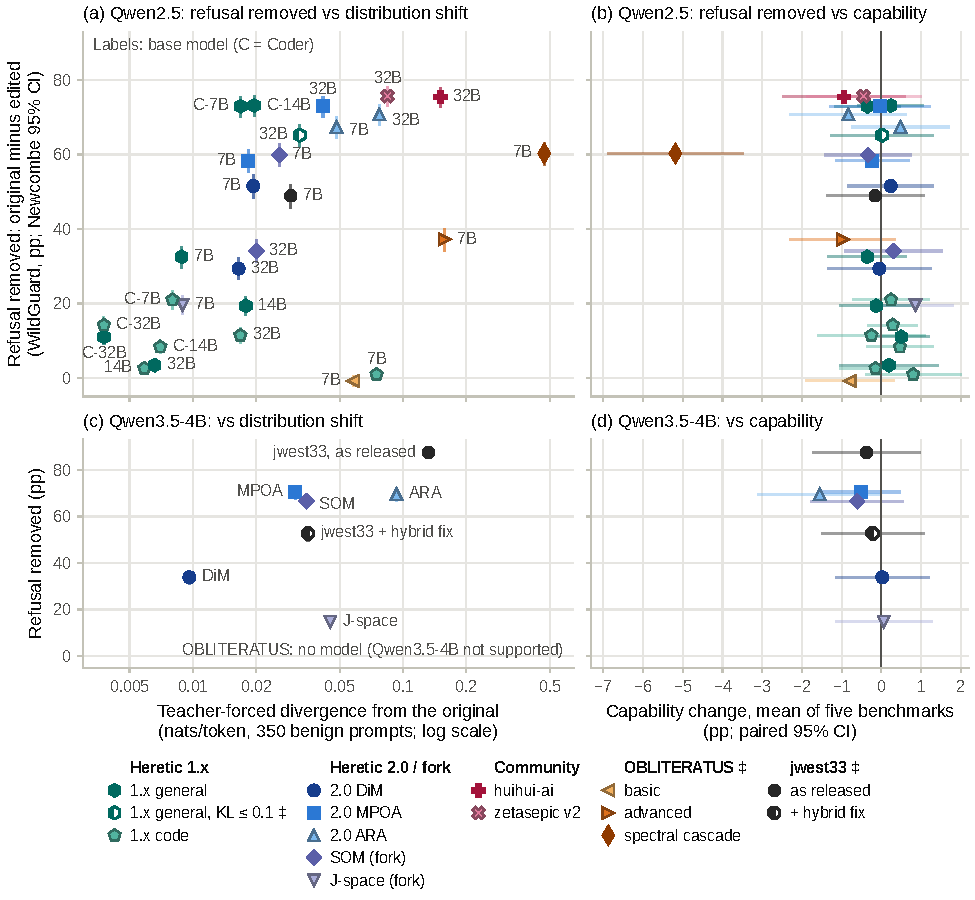
\includegraphics[width=\textwidth]{figures/fig2_tradeoff.pdf}
\caption{\textbf{Refusal removed versus its cost.} Each marker is one edited model. The vertical axis is the paired
reduction in WildGuard residual refusal from the model's own original (Newcombe 95\% CI). (a, c) TF divergence from
the original on the 350 benign held-out prompts (log scale). (b, d) Change of the mean of the five capability
benchmarks, with paired 95\% intervals. (a, b) Qwen2.5 models, labelled by base model (C = Coder), including the
cells added after the main design ($\S$: the KL $\le$ 0.1 re-export and the external tools on Qwen2.5-7B, each
external preset run once at its default or recommended settings); the jwest33 marker in (a, b) is the Qwen2.5-7B
run, whose runtime patch has no effect on that non-hybrid model, so it is effectively the tool as released. (c, d)
Qwen3.5-4B: the companion study's seed-1 models and the two jwest33 runs (as released, primary; with the hybrid
fix, sensitivity run); OBLITERATUS v0.1.4 does not support this model. The within-model correlations quoted here
use the main-design cells only (eight edited models on Qwen2.5-32B, seven on Qwen2.5-7B). Within Qwen2.5-32B, refusal removed rises with TF divergence (Spearman $\rho=-0.93$ for residual refusal);
within Qwen2.5-7B it does not ($\rho=-0.18$, not significant), because 1.x code moved that model furthest among the
Heretic models without removing refusal. Across base models the same divergence corresponds to very different
reductions (for example 11.4 to 73.1~pp between 0.016 and 0.021 nats per token), and at equal divergence tools can
differ (2.0 DiM versus 1.x code on Qwen2.5-32B). No capability change of the main design differs from zero; among
the added cells only OBLITERATUS \texttt{spectral\_cascade} ($-$5.18~pp) has an interval that excludes zero.
``(fork)'' = project-fork plug-in.}
\label{fig:tradeoff}
\end{figure*}

% src (cells.csv overrefusal_wg_rate; tests_refusal.csv vs_base benign_all wg 21/23; hb_harm_rate 32B and 7B)
Over-refusal on the benign prompts fell in 21 of the 23 edited models (Holm-significant); the exceptions were the 1.x
code variants on Qwen2.5-7B and Qwen2.5-14B. Harmful compliance by the HarmBench classifier mirrored refusal: on
Qwen2.5-32B it rose from 19.8\% for the original to 22.1\% and 27.6\% for the two 1.x variants, 40.3\% for 2.0 DiM,
82.3\% for ARA, 85.3\% for MPOA and 90.1\% and 91.0\% for the community releases; on Qwen2.5-7B from 23.3\% to 25.5\%
(1.x code), 45.6\% (1.x general) and 36.3\% to 79.0\% for the 2.0 and fork models.

\subsection{Search Records and the Selection Cap (Exploratory)}

% src (RESULTS.md "Dev set at matched KL caps"; dev_matched_kl.csv; correlations.csv dev_refusals_general~wg_rate
%      +0.95 [0.82, 1.00] n=15; cells.csv dev_refusals)
This section uses the optimisation records, not the held-out harness. Its counts are keyword refusals on the 100
dev prompts, scored during each search under that search's own settings: the 1.x searches used the
coding-assistant system prompt and 32 markers, the 2.0 and fork searches the generic system prompt and 33 markers
(Table~\ref{tab:h1setup}), so dev counts from the two versions are not directly comparable. Table~\ref{tab:devkl} and
Figure~\ref{fig:devkl} show what each search could have released at other dev-KL caps. At the 1.x cap (KL $\le$ 0.01)
the 1.x general search on Qwen2.5-32B had reached 89 dev refusals of 100, against 94 for 2.0 DiM, 83 for MPOA and 96
for SOM, while ARA had no trial below that cap. At the 2.0 cap (KL $\le$ 0.1) the same 1.x search had reached 50
(trial~\#96, the trial re-exported in \S\ref{sec:res-kl}), against 89 for DiM, 73 for SOM, 13 for MPOA and 10 for
ARA. On Qwen2.5-7B the 1.x general search reached 67 dev refusals at KL $\le$ 0.01, 30 at KL $\le$ 0.02 (ARA: 10) and
7 at KL $\le$ 0.1 (ARA 8, MPOA 19, SOM 27, DiM 55, J-space 84). At the 2.0 cap the 1.x general searches on the other
four models had reached 5 (Qwen2.5-Coder-7B), 9 (Qwen2.5-Coder-14B), 12 (Qwen2.5-14B) and 22 (Qwen2.5-Coder-32B)
dev refusals. The selected trials had realised dev KL of 0.004 to 0.010 (1.x) and 0.018 to 0.078 (2.0 and fork
plug-ins). Across the 15 edited models scored on the general dev prompts, the dev refusal count of the selected trial
ranked held-out residual refusal closely (Spearman $\rho=+0.95$ [0.82, 1.00]), but this pooled correlation mixes the
two dev protocols and six base models. Within Qwen2.5-32B, the selected 1.x general and 2.0 DiM trials both had 89
dev refusals and left 73.4\% and 47.4\% held-out residual refusal, and the re-exported 1.x trial with 50 dev
refusals left 11.6\%; within Qwen2.5-7B, the 1.x general and DiM trials had 67 and 55 dev refusals and left 39.6\%
and 20.6\%. Apart from trial~\#96, the held-out behaviour of unselected 1.x trials was not measured.

\begin{figure*}[tbp]
\centering
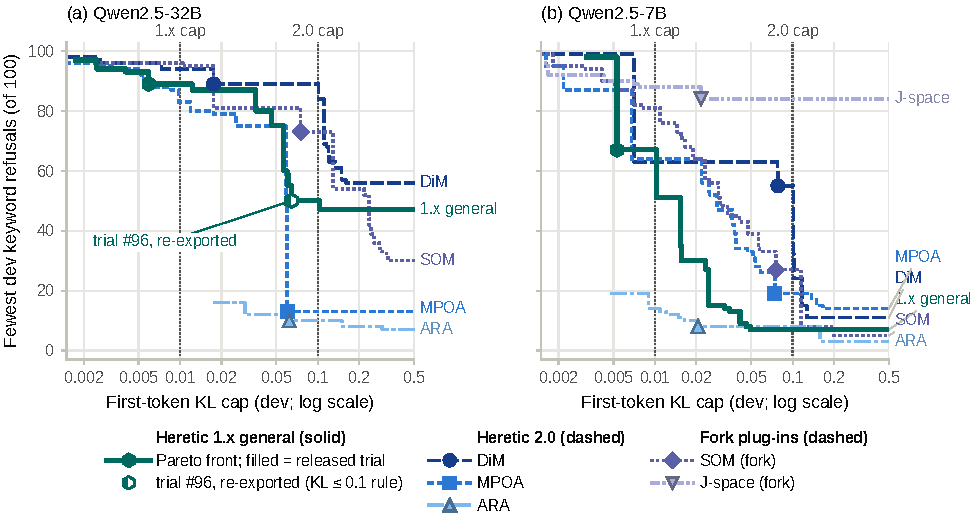
\includegraphics[width=\textwidth]{figures/fig4_dev_kl_budget.pdf}
\caption{\textbf{What each search could have released at a given dev-KL cap (search records; exploratory).}
Fewest keyword refusals among the 100 \texttt{harmful\_behaviors} dev prompts reached by any trial whose
first-token KL divergence is at or below the cap, for the Heretic~1.x general search (Pareto front of 200 trials,
seed~0) and the Heretic~2.0 and fork-plug-in searches (all 100 trials, seed~1). Dev counts were scored during each
search under its own settings (1.x: ``You are a helpful coding assistant.'', 32 markers; 2.0: ``You are a helpful
assistant.'', 33 markers), so the 1.x and 2.0 curves are not on a common scale. Filled markers: the released trial
(1.x: KL $\le$ 0.01 rule of the archived runs; 2.0 and fork: KL $\le$ 0.1 rule of the companion study); half-filled
hexagon in (a): 1.x trial~\#96, the trial that the KL $\le$ 0.1 rule selects, re-exported (\S\ref{sec:reexport}).
The 1.x code variant used a different dev set and is not shown. No held-out data enter this figure; the held-out
result of trial~\#96 is reported in \S\ref{sec:res-kl}.}
\label{fig:devkl}
\end{figure*}

\begin{table}[tbp]
\centering\small
\caption{Fewest dev keyword refusals (of 100 \texttt{harmful\_behaviors} test prompts) reachable at each
first-token KL cap, from the optimisation records (1.x: Pareto front; 2.0 and fork plug-ins: all trials);
``Selected'' is the released trial. Counts were scored under each search's own system prompt and marker list
(Table~\ref{tab:h1setup}) and are not directly comparable between 1.x and 2.0. -- = no trial at or below the cap.}
\label{tab:devkl}
\setlength{\tabcolsep}{4pt}
\resizebox{\textwidth}{!}{\begin{tabular}{@{}llrrrrrr@{}}
\toprule
Model & Search & Selected: refusals (KL) & \multicolumn{5}{c}{Fewest dev refusals at first-token KL $\le$} \\
\cmidrule(l){4-8}
 & & & 0.01 & 0.02 & 0.05 & 0.1 & 0.5 \\
\midrule
Qwen2.5-7B & 1.x general & 67 (0.005) & 67 & 30 & 7 & 7 & 7 \\
 & 2.0 DiM & 55 (0.078) & 63 & 63 & 63 & 55 & 11 \\
 & 2.0 MPOA & 19 (0.074) & 64 & 64 & 33 & 19 & 14 \\
 & SOM (fork plug-in) & 27 (0.076) & 81 & 64 & 39 & 27 & 5 \\
 & J-space (fork plug-in) & 84 (0.022) & 88 & 88 & 84 & 84 & 84 \\
 & 2.0 ARA & 8 (0.021) & 14 & 10 & 8 & 8 & 3 \\
\addlinespace[2pt]
Qwen2.5-Coder-7B & 1.x general & 21 (0.010) & 21 & 5 & 5 & 5 & 5 \\
\addlinespace[2pt]
Qwen2.5-14B & 1.x general & 91 (0.008) & 91 & 91 & 25 & 12 & 3 \\
\addlinespace[2pt]
Qwen2.5-Coder-14B & 1.x general & 36 (0.010) & 36 & 14 & 9 & 9 & 9 \\
\addlinespace[2pt]
Qwen2.5-32B & 1.x general & 89 (0.006) & 89 & 87 & 75 & 50$^{a}$ & 47 \\
 & 2.0 DiM & 89 (0.018) & 94 & 89 & 89 & 89 & 56 \\
 & 2.0 MPOA & 13 (0.060) & 83 & 79 & 75 & 13 & 13 \\
 & SOM (fork plug-in) & 73 (0.075) & 96 & 81 & 81 & 73 & 30 \\
 & 2.0 ARA & 10 (0.062) & -- & 16 & 12 & 10 & 7 \\
\addlinespace[2pt]
Qwen2.5-Coder-32B & 1.x general & 94 (0.007) & 94 & 86 & 74 & 22 & 4 \\
\bottomrule
\multicolumn{8}{@{}l}{\footnotesize $^{a}$ Trial \#96 (KL 0.064), re-exported and evaluated held-out (Table~\ref{tab:h1}b);} \\
\multicolumn{8}{@{}l}{\footnotesize \phantom{$^{a}$} dev re-evaluation after export: 51 of 100 at KL 0.064.} \\
\end{tabular}
}
\end{table}

\subsection{Summary of Findings}

The twelve Heretic~1.x models removed between 0.9~pp (not significant) and 73.1~pp of judged refusal, depending on
the base model and the direction source, with no detectable capability cost. In the pre-stated like-for-like
contrast, 2.0 DiM left less residual refusal than 1.x general on both base models (25.9~pp on Qwen2.5-32B, 19.0~pp
on Qwen2.5-7B), so H1 was supported as stated for the released checkpoints. When the archived 1.x general search on
Qwen2.5-32B was re-exported at the 2.0 selection rule, the 1.x model left 11.6\% of the harmful prompts refused:
61.7~pp less than the released export of the same search and 35.8~pp less than 2.0 DiM, at a TF divergence of 0.032
nats per token and without a detectable capability change; on that model only MPOA, ARA and the two community
releases left less. With both arms selected by the same rule, the like-for-like gap on Qwen2.5-32B therefore did not
persist (one search per arm; no such test exists for Qwen2.5-7B). A code-derived
direction gave no consistent advantage on malicious-code prompts in any of the six models (H2 not supported).
Keyword matching counted more refusals than the judge after strong edits, also within the first 256 tokens; within
the main design it rarely changed the order of tools, but among the external-tool contrasts it reversed one
significant difference (H3 partially supported). Of the external tools, each run once at its own default or
recommended settings, OBLITERATUS
\texttt{basic} removed no refusal, \texttt{advanced} removed 37.2~pp and \texttt{spectral\_cascade} 60.3~pp, the
latter with the only significant capability loss and the most degenerate responses in the study; jwest33's
abliterator removed 48.9~pp on Qwen2.5-7B and, as released, 87.4~pp on Qwen3.5-4B (52.7~pp with the
hybrid-architecture detection restored). Within Qwen2.5-32B, refusal removed tracked TF divergence closely; within
Qwen2.5-7B it did not.
